\renewcommand\thetable{\arabic{chapter}-\arabic{table}}
%\renewcommand\thefigure{\arabic{chapter}-\arabic{figure}}
\renewcommand{\theequation}{\arabic{chapter}-\arabic{equation}}
\chapter{Preliminaries}
\label{sec:preliminaries}

作業系統指紋辨識的方法,可分為主動式作業系統指紋辨識(Active OS Fingerprinting )與被動式作業系統指紋辨識(Passive OS Fingerprinting )。主動式作業系統指紋辨識,主動對目標主機送出自製的探測封包,並根據回傳的反應做判斷依據,軟體工具Nmap與Xprobe2即屬於此類。Nmap主要控制TCP的參數值,做為探測用封包;Xprobe2則是著重於送出ICMP 封包,利用邏輯樹斷定作業系統的類型。被動式作業系統指紋辨識是監聽網路上目標主機的封包往來做為判斷的依據,P0f即屬於被動式,相對於主動式作業系統指紋辨識較不易被人察覺。不論是主動式或被動式的作業系統指紋辨識,皆利用TCP/IP堆疊進行辨識,包括封包存活時間(time to live, TTL)、Window Size、最大分割大小(Maximum Segment Size)、不分段標記(Don't Fragment flag)、Window Scale Option等,因為不同的作業系統的fingerprint有所不同,所以可做為判定作業系統的依據。如圖~\ref{fig:PHI}所示。


\begin{figure}[t!]
  \begin{center}
    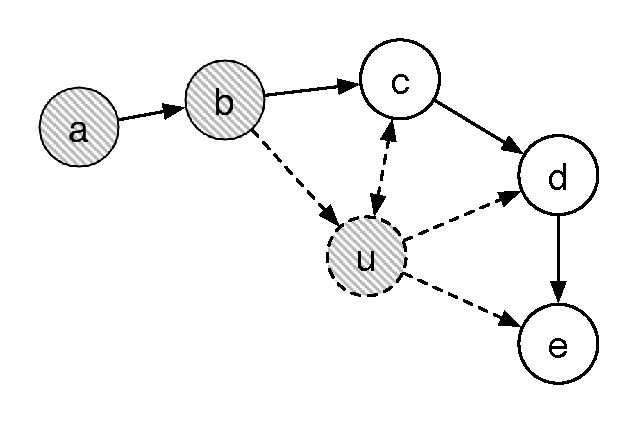
\includegraphics[width=1.0\textwidth]{figures/dyna_rm.eps}
    \caption{The diagram of ``prototypical PHI query''} 
    \label{fig:PHI}
  \end{center}
\end{figure}
